\documentclass[10pt,a4paper]{report}
\usepackage[utf8]{vietnam}
\usepackage{lmodern}
\usepackage{graphicx}
\usepackage{color}
\usepackage{hyperref}
\usepackage{amsmath}
\usepackage{amsfonts}
\usepackage{epstopdf}
\usepackage[table]{xcolor}
\usepackage{amsmath}
\usepackage{amsfonts}
\usepackage{amssymb}
\usepackage{multicol}
\usepackage{graphicx}
\usepackage{hyperref}
\usepackage{natbib}
\usepackage[left=2cm, right=2cm, top=2.00cm, bottom=2.00cm]{geometry}
\sloppy
\usepackage{tikz}
\usetikzlibrary{calc}
\newcommand\HRule{\rule{\textwidth}{1pt}}

\title{Báo cáo Thiết kế hệ thống số}
\author{Vũ Đức Cường - 20202313}

\usepackage{fancyhdr}
\pagestyle{fancy}
\fancyhf{}
\lhead{\large{\Large{T}}HIẾT {\Large{K}}Ế {\Large{H}}Ệ {\Large{T}}HỐNG {\Large{S}}Ố}
\rhead{\textbf{Project: Thực hiện phép cộng hai số có hai chữ số}}
\rfoot{Trang \thepage}
\lfoot{Vũ Đức Cường - Lê Xuân Đức - Đỗ Công Hiếu - Hoàng Anh Tú-}
\renewcommand{\footrulewidth}{0.4pt}




\begin{document}
	
	
	%% title page --------------------------------------
	\begin{titlepage}
		\begin{center}
			\begin{tikzpicture}[remember picture, overlay]
				\draw[line width = 2pt] ($(current page.north west) + (0.4in,-0.4in)$) rectangle ($(current page.south east) + (-0.4in,0.4in)$);
			\end{tikzpicture}
			{\LARGE{ \textbf{{\LARGE{Đ}}ẠI {\LARGE{H}}ỌC {\LARGE{B}}ÁCH {\LARGE{K}}HOA {\LARGE{H}}À {\LARGE{N}}ỘI}}}\\
			\vspace{0.5cm}
			{\large{\textbf{TRƯỜNG ĐIỆN - ĐIỆN TỬ}}}\\
			\vspace{0.5cm}
			\large{\textbf{Khoa Tự động hóa}}\\
			\vspace{2cm}
			
\includegraphics[scale=0.2]{LoGo}\\
			\vspace{1cm}
			{\LARGE{ \textbf{Thiết kế mạch cộng hai số có hai chữ số\\ \vspace{0.3cm} điều chỉnh bằng nút nhấn và hiển thị trên LED 7 thanh}}}\\
			\vspace{2cm}
			\textbf{\begin{tabular}{ l l l}
					Họ và tên sinh viên: & Vũ Đức Cường \quad & 20202313 \\
					\qquad & \qquad &\\
					\qquad & \ Lê Xuân Đức& 20191759\\
					\qquad & \qquad &\\
					\qquad & Đỗ Công Hiếu & 20202620 \\
					\qquad & \qquad &\\
					\qquad & Hoàng Anh Tú& 20164460\\
					\qquad & \qquad &\\
					Giảng viên hướng dẫn: \qquad \qquad & Nguyễn Cảnh Quang  &\\
					\qquad & \qquad &\\
					Mã lớp học:\qquad\qquad\qquad & 133186 & \\
			\end{tabular}}\\
			\vspace{2cm}
			{\large{\textbf{HÀ NỘI, 5/2022}}}\\
		\end{center}
	\end{titlepage}



%% Lời nói đầu
\addcontentsline{toc}{section}{Lời nói đầu}
\textbf{{\LARGE{Lời nói đầu}}}
Trong thời kỳ hội nhập và xu thế cuộc cách mạng công nghiệp 4.0, Việt Nam đang là một trong những nước tích cực thực hiện công nghiệp hóa nhất trong khu vực. Chúng ta đang đẩy mạnh việc ứng dụng các nguồn năng lượng tái tạo, xây dựng các khu công nghệ, khu công nghiệp hiện đại với nhiều dây chuyền sản xuất có tính tự động hóa cao. Để đáp ứng được mục tiêu đó cần có nguồn nhân lực chuyên môn sâu về lĩnh vực Tự động hóa. Trong những năm gần đây, với sự phát triển không ngừng và những thành tựu đáng kể từ khắp nơi trên thế giới về vi mạch, vi xử lý (chip) và kỹ thuật số (digital) đòi hỏi sinh viên ngành Tự động hóa phải chủ động bắt kịp, tìm kiếm và khai thác những kiến thức mới, từ đó tiếp cận và làm chủ các công nghệ hiện đại đáp ứng được các yêu cầu sản xuất. Để có thể đạt được mục tiêu đó trước hết sinh viên cần phải nắm vững những kiến thức căn bản về điện tử số mà môn học Thiết kế hệ thống số đóng vai trò quan trọng. 
Môn học Thiết kế hệ thống số giúp sinh viên rèn luyện kỹ năng hệ thống các  thiết kế với sự hỗ trợ của các công cụ, làm việc theo nhóm và tổng hợp thiết kế cuối cùng. Trên cơ sở các kiến thức cơ bản này sẽ nhằm tạo tiền đề cho những môn học kế tiếp cũng như giúp sinh viên tiếp cận các vấn đề hiện đại, đồng thời liên hệ với thực tế kỹ thuật, từ đó giúp sinh viên nắm vũng được những vấn đề cốt lõi của kỹ thuật điện tử số, tăng cường khả năng giải quyết các vấn đề kỹ thuật trong thực tế.
Với mục đích trau dồi và bổ sung thêm kiến thức về môn học, nhóm chúng em đã tiến hành nghiên cứu và thực hiện project mang tên “Thiết kế mạch cộng hai số có hai chữ số điều chỉnh bằng nút nhấn và hiển thị trên LED 7 thanh” để có thể áp dụng những kiến thức từ môn học thành một sản phẩm kỹ thuật điện tử số có tính ứng dụng.\\

Trong quá trình thực hiện project không tránh khỏi những thiếu sót, chúng em rất mong nhận được sự phê bình, đóng góp từ thầy cũng như các bạn. Chúng em xin chân thành cảm ơn.



\begin{flushleft}
	Hà Nội, ngày 12/07/2022

Nhóm tác giả
\end{flushleft}







\newpage 
%% Mục lục
\tableofcontents
\newpage



\chapter{Tổng quan bài toán}

\hspace{0.3cm} Thiết kế hệ thống số để cộng 2 số có 2 chữ số.\\

Bài toán cộng có lẽ không phải là một bài toán quá xa lạ với chúng ta khi nó xuất hiện hằng ngày trong đời sống. Hiện nay có rất nhiều công cụ để xử lý phép toán cộng (vi xử lý, các máy tính nhúng, ...). \\
Và trong môn học \textbf{Thiết kế hệ thống số}, thì em sẽ trình thuật toán, quy trình để thiết kế một hệ thống chỉ sử dụng các IC số có thể tính toán và hiển thị được phép tính cộng trên LED 7 thanh.\\

Hệ thống có đầu vào là các nút nhấn, đầu ra (tức kết quả) được hiển thị trên LED 7 đoạn.\\
\begin{center}
	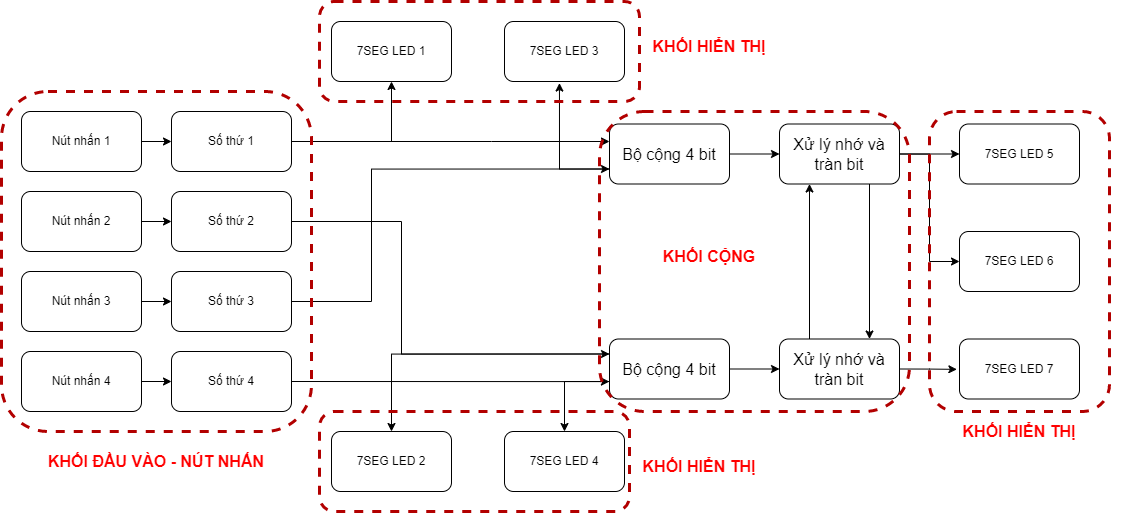
\includegraphics[width=0.9\linewidth]{sodo}
\end{center}

Giao diện tổng quan của bo mạch\\
\begin{center}
	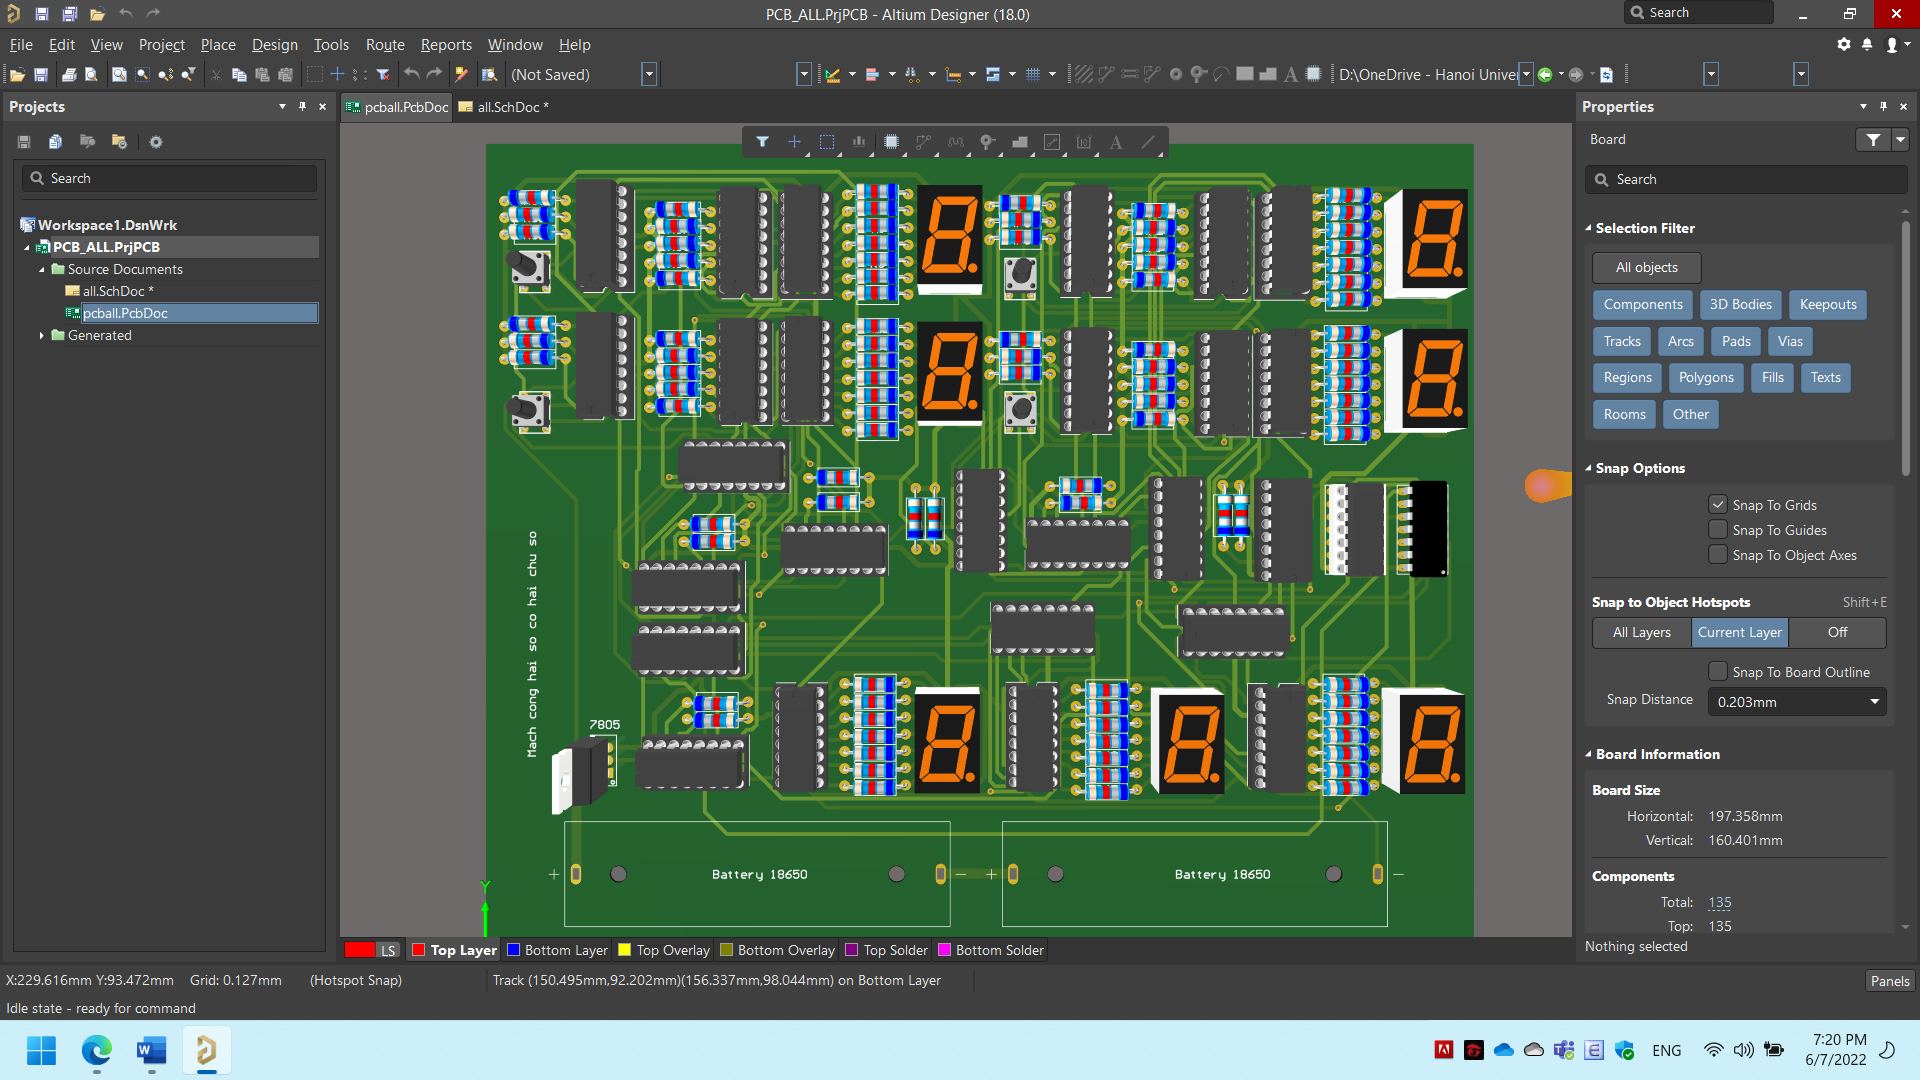
\includegraphics[width=0.7\linewidth]{img_all}
\end{center}
\vspace{1cm}

\textbf{Đầu vào} là 4 nút nhấn (SW1, SW2, SW3, SW4) để điều khiển 4 LED 7 đoạn.
\begin{itemize}
	\item SW1: điều khiển hàng chục của số hạng thứ nhất.
	\item SW2: điều khiển hàng đơn vị của số hạng thứ nhất.
	\item SW3: điều khiển hàng chục của số hạng thứ thứ hai.
	\item SW4: điều khiển hàng đơn vị của số hạng thứ hai.
\end{itemize}

Mỗi lần nhấn nút thì giá trị của mỗi LED tăng lên 1 đơn vị (0 $\to$ 1 $\to$ 2 $\to$ ... $\to$ 9 $\to$ 0 )\\

\textbf{Phần trung tâm xử lý} bao gồm các IC số (IC cộng 4 bits, IC so sánh 4 bits, IC JKFlipFlop, IC chuyển đổi BCD ra LED 7 thanh, ...)\\

\textbf{Đầu ra} là 7 LED 7 thanh để hiển thị các số hạng và kết quả của phép toán cộng giữa hai số hạng.
\begin{itemize}
	\item LED1: Hiện thị hàng chục của số hạng thứ nhất.
	\item LED2: Hiển thị hàng đơn vị của số hạng thứ nhất.
	\item LED3: Hiển thị hàng chục của số hạng thứ thứ hai.
	\item LED4: Hiển thị hàng đơn vị của số hạng thứ hai.
	\item LED5: Hiển thị hàng trăm của kết quả.
	\item LED6: Hiển thị hàng chục của kết quả.
	\item LED7: Hiển thị hàng đơn vị của kết quả.
\end{itemize}

\textbf{Nguồn} điện áp cấp là 5VDC\\

\newpage
\chapter{Thực hiện}
\section{Thực hiện phép cộng 2 số có 2 chữ số}
\subsection{Cách thực hiện phép cộng số có 2 chữ số với mã nhị phân}

\hspace{0.3cm} Bài toán đặt ra yêu cầu là thực hiện phép cộng 2 chữ số (kết quả có thể là 3 chữ số) thì ta cần ít nhất 1byte = 8bits để biểu diễn số lớn nhất của phép cộng 99 + 99 = 198 (1100 0110). Việc thực hiện trên 8 bit là rất vất vả, và hiển thị ra LED 7 đoạn là một bài toán dài và khó. Thế nên ở đây ta sẽ chỉ làm việc với 4bits, bởi các IC 4bits có giá cả rẻ hơn và dễ thực hiện hơn.\\

Quay trở lại bài toán lớp 1, ta đã biết cách thực hiện phép cộng như sau:
\begin{center}
	\includegraphics[width=0.3\linewidth]{image/phepcong}
\end{center}

Ở đây, ta thực hiện cộng hàng đơn vị với hàng đơn vị, nếu có nhớ, chuyển sang hàng tiếp theo, đến khi thực hiện hết. Phép tính được làm tuần tự từ phải qua trái, và thực hiện tuần tự từ hàng nọ sang hàng kia.\\

Ta sẽ biểu diễn mã nhị phân theo kiểu BCD (Binary Code Decimal). Tức là một số có $n$ chữ số sẽ cần $4n$ bits.\\

\textbf{Ví dụ: } Số 13 trong mã thập phân nếu biểu thị theo kiểu BCD sẽ là: 0001 (1) 0010 (3)\\

Phép cộng sẽ thực hiện với 4 bits, cộng từng hàng cả các số hạng với nhau. Nếu xảy ra tràn bit (tức là phép cộng hai số có kết quả lớn hơn 15), lúc đó ta sẽ sử dụng đến bit nhớ, tức là phép tính có kết quả là 5 bits.\\

Tuy nhiên, kết quả cần khi cộng hai hàng vào với nhau phải là số có 1 chữ số, nên phải trừ đi 10, và nhớ 1 sang hàng sau. Thế khi nào thực hiện phép trừ 10, khi mà có phần dư, tức là khi tràn bit, hoặc là lớn hơn 10.\\

Tràn bit và lớn hơn 10 hoàn toàn khác nhau, lớn hơn 10 chưa chắc đã tràn bit, và tràn bit chưa chắc đã lớn hơn 10. Lấy một ví dụ thực hiện phép cộng như sau:
\begin{align}
	& 9 \to (0) 1001 \notag \\
	& 7 \to (0) 0111 \notag \\
	1&6 \to (1) 0000 \quad \text{Đã xảy ra tràn bit}
\end{align}

Như trên, ta thấy đã xảy ra tràn bit, tuy nhiên, kết quả của phép tính thực hiện được lại là 0 < 10 (bài toán đang thực hiện trên 4 bits). Thế nên, ta cần một điều kiện hoặc để biết khi nào kết quả nhận được khi cộng hai hàng tương ứng ra một số lớn hơn 10.

Chẳng hạn như phép tính bên trên thực hiện trên hàng đơn vị của một phép tính giữa 2 số hạng có 2 chữ số, thì kết quả ta cần là số 6. Thực hiện phép tính trừ 10, tức là cộng 4 bits kết quả với bù 2 của 10 (0110) trong hệ nhị phân ta sẽ thu được số 6.\\

Tương tự với hàng chục ta sẽ có được kết quả!

\subsection{Bộ cộng full 4 bits - 74LS83}

Đọc tham khảo Data Sheet của Bộ cộng full 4bits tại đây: \hyperref{https://pdf1.alldatasheet.com/datasheet-pdf/view/51091/FAIRCHILD/74LS83.html}{category}{name}{Data Sheet 74LS83} %\cite{74LS83}\\

\textbf{Sơ đồ chân của IC 74LS83}
\begin{center}
	\includegraphics[width=0.6\linewidth]{image/74ls83}
\end{center}

Chi tiết sơ đồ chân:
\begin{itemize}
	\item IC có tổng cộng 16 chân
	\item Chân số 5 và 12 được sử dụng để cấp nguồn 5VDC cho IC
	\item Giả sử có hai số có 4bits A4 A3 A2 A1 (tương ứng với các chân đầu vào là 1, 3, 8, 10)và B4 B3 B2 B1 (tương ứng với các chân đầu vào là 16, 4, 7, 11) với B1 và A1 là LSB (bit có trọng số nhỏ nhất) thì kết quả của phép cộng là S4 S3 S2 S1 được xuất qua các chân tương ứng là 15, 2, 6, 9.
	\item Chân 13 là một chân đầu vào Carry in (phần nhớ của phép tình trước sẽ được thêm vào đây). Tuy nhiên, điều này sẽ chỉ làm bài toán của mình trở nên phức tạp, thế nên các phép tính sẽ được làm mà không có Carry in.
	\item Chân 14 là chân đầu ra kết quả bit nhớ của phép tính (xảy ra tràn bit xung của chân này sẽ kích lên mức cao)
\end{itemize}

\textbf{Bảng sự thật của IC:}

\begin{center}
		\includegraphics[width=0.7\linewidth]{image/bangsuthat7483}

\end{center}

\textbf{Sơ đồ logic bên trong IC:}
\begin{center}
	\includegraphics[width=0.5\linewidth]{image/sodoLogic7483}
\end{center}

\textbf{Mô phỏng trong Proteus:}
\begin{center}
	\includegraphics[width=1\linewidth]{image/prt7483}
\end{center}

\vspace{2cm}
\subsection{Bộ so sánh 4 bits - 74LS85}

Đọc tham khảo Data Sheet của Bộ so sánh tại đây: \hyperref{https://pdf1.alldatasheet.com/datasheet-pdf/view/12664/ONSEMI/74LS85.html}{category}{name}{Data Sheet 74LS85} %\cite{74LS85}\\

\textbf{Sơ đồ chân của IC:}
\begin{center}
	\includegraphics[width=0.7\linewidth]{image/74ls85}
\end{center}

Chi tiết sơ đồ chân:
\begin{itemize}
	\item IC có tất cả 16 chân
	\item Các chân đầu vào bao gồm các chân 10, 12, 13, 15 tương ứng với các bit A0 (LSB), A1, A2, A3 (MSB) của số thứ nhất và các chân 9, 11, 14, 1 tương ứng với các bit B0 (LSB), B1, B2, B3 (MSB) của số thứ hai. 
	\item Các chân đầu vào 2, 3, 4 sẽ không được sử dụng trong phạm vi bài báo cáo này.
	\item Chân đầu ra 5 (OA>B) sẽ được kích mức HIGH nếu A > B
	\item Tương tự với 2 chân đầu ra 5 và 6
	\item Các chân cấp điện áp 8 (GND) và 16 (VCC) được dùng để cấp điện áp cho IC.
\end{itemize}

\begin{multicols}{2}
	\textbf{Sơ đồ logic bên trong IC: }
	\begin{center}
		\includegraphics[width=1\linewidth]{image/sodoLogic7485}
	\end{center}
	
	
	\textbf{Bảng sự thật của IC:}
	\begin{center}
		\includegraphics[width=1\linewidth]{image/bangsuthat7485}
	\end{center}
\end{multicols}


\textbf{Mô phỏng Proteus: }
\begin{center}
	\includegraphics[width=0.5\linewidth]{image/prt7485}
\end{center}

\vspace{2cm}

\subsection{Sơ đồ nguyên lý của mạch cộng hai số có hai chữ số}
\begin{center}
	\includegraphics[width=1\linewidth]{image/machcong}
\end{center}

\newpage
\section{Hiển thị}
\subsection{LED 7 đoạn}
\begin{center}
	\includegraphics[width=0.7\linewidth]{image/led7doan}
\end{center}

Led 7 thanh (7-segment Display) hay còn được gọi là led 7 đoạn được thiết kế để hiển thị số và một số ký hiệu khác %\cite{LED}. LED 7 đoạn có 2 loại là loại Catot chung và Anot chung (âm chung và dương chung).\\

Cấu tạo của LED 7 đoạn là 7 LED đơn, có hình dáng là mỗi đoạn a, b, c, d, c, d, e, f, g, dp. Để hiện thị một số lên trên màn hình, đối với loại Anot chung, thì sẽ nối đất Catot của mỗi LED đơn trong LED 7 đoạn, còn đối với loại Katot chung thì sẽ nối dương Anot của mỗi LED đơn trong LED 7 đoạn.\\
\begin{center}
	\includegraphics[width=1\linewidth]{image/led7doan_hienthi}
\end{center}

Ta có bảng sự thật của LED 7 đoạn Anode chung như sau:
\begin{center}
	\includegraphics[width=0.8\linewidth]{image/anotchungled}
\end{center}

\textbf{Mô phỏng Proteus: } đối với LED 7 đoạn Anode chung
\begin{center}
	\includegraphics[width=0.7\linewidth]{image/prtled7ca}
\end{center}

\vspace{2cm}
\subsection{IC giải mã BCD sang LED 7 đoạn - 74LS247}
Tham khảo Data Sheet của IC giải mã BCD sang LED 7 đoạn tại đây: \hyperref{https://pdf1.alldatasheet.com/datasheet-pdf/view/12641/ONSEMI/74LS247.html}{category}{name}{Data Sheet 74LS247} %\cite{74LS247}\\

Như đã biết, kết quả của phép cộng là 3 chữ số, mỗi chữ số được biểu diễn bằng một mã 4 bits (Biểu diễn theo kiểu BCD), và LED 7 đoạn có vai trò hiển thị từng chữ số đó lên. Thế nên ở đây ta cần một IC có khả năng làm được việc đó, giải mã BCD sang mã LED 7 đoạn.\\

\textbf{Sơ đồ chân của IC 74LS247:}
\begin{center}
	\includegraphics[width=0.6\linewidth]{image/74ls247}
\end{center}

Chi tiết sơ đồ chân của IC:
\begin{itemize}
	\item IC có tất cả 16 chân, rất dễ sử dụng
	\item Chân cấp nguồn: 16 (VCC) và 8 (GND)
	\item Chân đầu vào: 7, 1, 2, 6 tương ứng với 4 bits A(LSB), B, C, D (MSB).
	\item Chân đầu ra 13, 12, 11, 10, 9, 15, 14 tương ứng với các chân của LED 7 thanh là a, b, c, d, e, f, g
\end{itemize}

\textbf{Sơ đồ logic của IC: }
\begin{center}
	\includegraphics[width=0.7\linewidth]{image/sodoLogic74247}
\end{center}

\textbf{Bảng sự thật của IC:}
\begin{center}
	\includegraphics[width=0.8\linewidth]{image/bangsuthat74247}
\end{center}

\textbf{Mô phỏng Proteus: }
\begin{center}
	\includegraphics[width=0.5\linewidth]{image/prt74247}
\end{center}
\subsection{Sơ đồ nguyên lý khối hiển thị}
\begin{center}
	\includegraphics[width=0.7\linewidth]{image/sodonguyenlykhoicong}
\end{center}


\newpage
\section{Đầu vào - Nút nhấn}
\hspace{0.3cm} Mỗi nút nhấn đóng vai trò điều khiển 1 LED 7 đoạn, mỗi lần nhấn nút, giá trị hiển thị trên mỗi LED 7 đoạn sẽ tăng một đơn vị.\\

\subsection{74LS76 JK Flip-Flop kép}
Đọc tham khảo Data Sheet của IC 74LS76 tại đây: \hyperref{https://pdf1.alldatasheet.com/datasheet-pdf/view/12663/ONSEMI/74LS76.html}{category}{name}{Data Sheet 74LS76 JK Flip-Flop} %\cite{74LS76}
\begin{center}
	\includegraphics[width=0.7\linewidth]{image/74ls76}
\end{center}

Chi tiết sơ đồ chân: %\cite{flipflop}
\begin{itemize}
	\item Chân 1 (1 CLK): là chân đầu vào. Nó được sử dụng để cung cấp xung nhịp cho flip flop JK đầu tiên. Xung mức CAO đến THẤP sẽ tác động đến flip flop.
	\item Chân 2 (1 PRE'): là chân đầu vào preset. Nó được sử dụng để preset (1Q) của flip flop đầu tiên lên mức CAO. Là chân tích cực mức thấp.
	\item Chân 3 (1 CLR'): là chân đầu vào Clear của flipflop đầu tiên. Nó được sử dụng để reset đầu ra của flip flop đầu tiên. Nó là chân tích cực mức thấp.
	\item Chân 4 (CLR'): là chân đầu vào đầu tiên của flipflop đầu tiên. Nó được sử dụng để nhận bit dữ liệu đầu vào đầu tiên cho vi mạch. Nó có thể là mức CAO hoặc THẤP.
	\item Chân 4 (1 J): là chân đầu vào đầu tiên của flipflop đầu tiên. Nó được sử dụng để nhận bit dữ liệu đầu vào đầu tiên cho vi mạch. Nó có thể là mức CAO hoặc THẤP.
	\item Chân 5 (VCC): được sử dụng làm chân nguồn. Nó được sử dụng để cấp nguồn cho vi mạch cho nó hoạt động.
	\item Chân 6 (2 CLK): là một chân đầu vào. Nó được sử dụng để cấp xung clock cho flip flop JK thứ hai. Xung mức CAO đến THẤP sẽ có tác động đến vi mạch.
	\item Chân 7 (2 PRE'): là chân đầu vào preset của flip flop thứ hai. Nó được sử dụng để làm cho đầu ra (2Q) của flip flop thứ hai lên mức cao. Là chân tích cực mức thấp.
	\item Chân 8 (CLR'): là chân đầu vào clear của flip flop thứ hai. Nó được sử dụng để reset lại đầu ra của flip flop thứ hai. Là chân tích cực mức thấp.
	\item Chân 9 (2 J): là chân đầu vào đầu tiên của flipflop thứ hai. Nó được sử dụng để cấp bit dữ liệu đầu vào đầu tiên cho vi mạch. Nó có thể là mức CAO hoặc THẤP.
	\item Chân 10 (2 Q'): là chân đầu ra thứ hai của flip flop thứ hai. Nó sẽ cung cấp đầu ra đảo ở chân 11.
	\item Chân 11 (2 Q): là chân đầu ra đầu tiên của flipflop thứ hai. Nó kích bit đầu ra của flip flop thứ hai.
	\item Chân 12 (2 K): là chân đầu ra đầu tiên của flipflop thứ hai. Nó kích bit đầu ra của flip flop thứ hai.
	\item Chân 13 (GND)
	\item Chân 14 (1 Q'): là chân đầu ra thứ hai của flip flop đầu tiên. Nó sẽ cấp đầu ra đảo ở chân 15.
	\item Chân 15 (1 Q): là chân đầu ra đầu tiên của flip flop đầu tiên. Nó sẽ cấp bit đầu ra của flip flop đầu tiên.
	\item Chân 16 (1 K): là chân đầu ra đầu tiên của flip flop đầu tiên. Nó sẽ cấp bit đầu ra của flip flop đầu tiên.
\end{itemize}

\textbf{Sơ đồ Logic của IC: }
\begin{center}
	\includegraphics[width=0.8\linewidth]{image/logic74ls76}
\end{center}

\textbf{Bảng sự thật của IC: }
\begin{center}
	\includegraphics[width=0.7\linewidth]{image/bangsuthat7476}
\end{center}
 \textbf{Mô phỏng Proteus: }

\begin{center}
	 	\includegraphics[width=0.7\linewidth]{image/prt7476}
\end{center}

Do đây là một bộ đếm với 4 bits, nên nó sẽ đến từ 0000 cho đến 1111. Vậy nên ở đây ta cần dùng một bộ so sánh để Reset lại bộ đếm quay ngược trở về 0 khi đếm đến 10. Bộ so sánh đã được trình bày ở trên, Mục \textbf{2.1.3. Bộ so sánh 4 bits - 74LS85}

\subsection{Sơ đồ nguyên lý của khối nút nhấn} 
\begin{center}
	\includegraphics[width=1\linewidth]{image/sodonguyenlynutnhan}
\end{center}


\newpage
\chapter{Kết quả - Gỡ lỗi}
\section{Thực hiện mô phỏng trên Proteus}
Thực hiện mô phỏng trên Proteus sau khi kết nối các khối với nhau cho được kết quả chính xác đúng như lý thuyết
\begin{center}
	\includegraphics[width=1\linewidth]{image/prtfull}
\end{center}
\vspace{1cm}
\begin{center}
	\includegraphics[width=1\linewidth]{image/prtfull2}\\
	\textbf{\textit{Thực hiện phép cộng không nhớ}}
\end{center}
\vspace{1cm}
\begin{center}
	\includegraphics[width=1\linewidth]{image/prtfull3}\\
	\textbf{\textit{Thực hiện phép cộng có nhớ với hàng đơn vị}}
\end{center}
\vspace{1cm}
\begin{center}
	\includegraphics[width=1\linewidth]{image/prtfull4}\\
	\textbf{\textit{Thực hiện phép cộng có nhớ với cả 2 hàng}}
\end{center}
\newpage
\section{Thiết kế, hàn mạch cứng}
\begin{itemize}
	\item Mạch được vẽ trên phần mềm Altium, do sửa mạch nhưng quên backup nên chỉ còn lại file Gerber gửi đi gia công
	\item Mạch được đặt gia công bởi 1 xưởng gia công trong nước.
\end{itemize}
\begin{multicols}{2}
\begin{center}
	\includegraphics[height=5cm]{image/geber}\\
	\textbf{\textit{File Gerber}}
\end{center}

\begin{center}
	\includegraphics[height=5cm]{image/machin}\\
	\textbf{\textit{Kết quả mạch in}}
\end{center}
\end{multicols}
\vspace{2cm}
Kết quả thực hiện trên mạch cứng
\begin{center}
	\includegraphics[width=0.6\linewidth]{image/real}\\
	\textbf{\textit{Thực hiện phép tính trên mạch thật}}
\end{center}
\newpage
\section{Gỡ lỗi}

\textbf{Lỗi về nguồn}
\begin{itemize}
	\item Sử dụng 2 pin 18650 $\to U \approx 8V$, qua ổn áp bằng IC7805, tuy nhiên IC không chịu được dòng lớn, và quá tải.
	\item  Sử dụng 2 pin 18650 $\to U \approx 8V$, không qua ổn áp, gây ra dòng lớn ~1.2A, các đường dây bị nóng, IC, trở bị nóng. Điều này giảm tuổi thọ cho IC.
	\item  Sử dụng 1 pin 18650, $\to U \approx 4.2V$, mạch hoạt động bình thường ở điện áp thấp hơn điện áp định mức. Tuy nhiêm, sụt áp không đáng kể và các điện áp mức cao khi đến chân IC vẫn lớn hơn 3.3V
\end{itemize}
\vspace{1cm}
\textbf{Lỗi đi dây trong mạch}
\begin{multicols}{2}
	\begin{center}
		\includegraphics[width=0.9\linewidth]{image/bug1}\\
		\textbf{\textit{Lỗi không kéo nút nhấn lên 5V}}
	\end{center}
	\begin{center}
		\includegraphics[width=0.9\linewidth]{image/bug2}\\
		\textit{\textbf{Lỗi không kéo Pre-set lên 5V}}
	\end{center}
	\begin{center}
		\includegraphics[width=0.9\linewidth]{image/bug5}\\
		\textbf{\textit{Lỗi vẽ sai Schematic trong Altium}}
	\end{center}
	\begin{center}
		\includegraphics[width=0.9\linewidth]{image/bug4}\\
		\textbf{\textit{Lỗi vẽ sai Schematic trong Altium}}
	\end{center}
\end{multicols}
\vspace{1cm}
\begin{flushleft}
	\textbf{Mạch FlipFlop hoạt động không ổn định}: Mạch Flip Flop hoạt động không ổn định có các nguyên nhân sau:
\end{flushleft}
\begin{itemize}
	\item Chân IC bị lỏng, IC kém chất lượng, gây ra nhiễu trong quá trình sử dụng. Trong quá trình kiểm tra, có những lúc Q và $\overline{Q}$ có cùng mức logic nhưng 2 chân này không thông mạch.
	\item Do nhấn hiện tượng dội nút nhấn, nhấn 1 lần FF nhận là nhấn nhiều lần, hoặc nhấn nhiều lần mà FF không nhận được (do thời gian quá độ của xung)
\end{itemize}
\begin{multicols}{2}
	\begin{center}
		\includegraphics[width=\linewidth]{image/bug7}
	\end{center}
	$\to$ Các xung xuất hiện trong thời gian rất ngắn, trong khi thiết bị không đủ nhạy, mắt người không đủ khả năng để quan sát nên rất khó phát hiện.\\
	Hình ảnh bên là một lần may mắn thu lại được tín hiệu
\end{multicols}

\begin{flushleft}
	\textbf{Thiếu trường hợp trong Schematic}
\end{flushleft}
Trong quá trình mô phỏng, tại xử lý bit bị tràn đã quên đi mất phải OR bit bị tràn và bit lớn hơn bằng 10 với nhau để tạo ra bit số hàng trăm. Đây là một lỗi dễ sửa, chỉ cần sử dụng con OR còn lại trong IC 74HC32 để làm phép tính là có thể ra được bit đưa vào hàng trăm
\begin{multicols}{2}
	\begin{center}
		\includegraphics[width=0.9\linewidth]{image/bug3}\\
		\textbf{\textit{Đi dây lại cho 74HC32}}
	\end{center}
	\hfill\null\columnbreak
	\begin{center}
		\includegraphics[width=0.9\linewidth]{image/bug6}\\
		\textbf{\textit{Sử dụng thêm partD của IC để thực hiện phép OR còn lại}}
	\end{center}
\end{multicols}







\newpage
\addcontentsline{toc}{chapter}{Tài liệu}

\begin{thebibliography}{9}
	\bibitem{74LS83}
	Fairchild Semiconductor Corporation (Aug, 1986), \textit{DM74LS83A4-Bit Binary Adder with Fast Carry}
	
	\bibitem{74LS85}
	Semiconductor Components Industries (Dec, 1999), \textit{SN74LS854 - Bit Magnitude Comparator}
	
	\bibitem{LED}
	Website: {https://dientusangtaovn.com}, \textit{https://dientusangtaovn.com/led-7-thanh-la-gi/}
	
	\bibitem{74LS247}
	Semiconductor Components Industries (Dec, 1999), \textit{SN74LS247 - BCD to Seven Segment Decoders/Drivers}
	
	\bibitem{74LS76}
	Semiconductor Components Industries (Dec, 1999), \textit{SN74LS76 - Dual JK Flip-Flop with Set and Clear}
	
	\bibitem{flipflop}
	https://blog.mecsu.vn, \textit{https://blog.mecsu.vn/74ls76-jk-flip-flops-kep-co-chuc-nang-preset-va-clear}
\end{thebibliography}


\end{document}